\documentclass[a4paper]{article}

\usepackage[english]{babel}
\usepackage[utf8]{inputenc}
\usepackage{amsmath}
\usepackage{graphicx}
\usepackage[colorinlistoftodos]{todonotes}
\usepackage{tipa}
\usepackage{float}

\title{LING 401: Milestone 4}

\author{Guohao Dou}

\date{\today}

\begin{document}
\maketitle

\section{Vowel Qualities}
\subsection{Overview}

The first 100 words in Cantonese Swadesh list was read by a native speaker of Cantonese and recorded in an ideal environment. There are 7 distinguishable vowels (o, i, a, u, e, y, œ) present in the small corpus. It should be noted that [a\textlengthmark] is also present. However, according to the criteria discussed in WALS, [a\textlengthmark] is not counted in the 7 vowel types. Moreover, there's no significant difference in formant values between [a] and [a\textlengthmark], meaning that duration and loudness, instead of formant values, may be adopted to contrast [a] and [a\textlengthmark]. 

The following policy is adopted to handle diphthongs. Since there are three points of measurement for any acoustic feature (f0, F1, F2, and F3), the first of the three gets assigned to the first phoneme in a diphthong and the last gets assigned to the second phoneme. Also, when measuring vowel duration, diphthongs are simply discarded since it is difficult to find a clear cut. 

\subsection{Vowel Duration}
The table below contains the average and standard deviation of the duration of the seven vowel types as well as [a\textlengthmark]. 

\begin{table}[!htbp]
    \begin{tabular}{|c|c|c|c|c|c|c|c|c|}
        \hline
         & i & u & a & e & o & y & œ & a\textlengthmark\\
        \hline
        \# of occurrence & 13 & 3 & 17 & 7 & 18 & 7 & 3 & 13\\
        \hline
        mean duration(s) & 0.1488 & 0.1002 & 0.08601 & 0.1026 & 0.1179 & 0.1481 & 0.1844 & 0.1561\\
        \hline
        standard deviation & 0.05925 & 0.03360 & 0.03480 & 0.03199 & 0.05812 & 0.05625 & 0.03097 & 0.03422\\
        \hline
    \end{tabular}
\end{table}
As we can see, statistically [a\textlengthmark] has a longer duration than [a]. However, since the sample size is quite small for most phonemes, more conclusions cannot be easily drawn. 

\subsection{Formant Frequencies}
This section includes spectrograms for the seven vowel types.
% TODO: uncomment before submitting
% \begin{figure}[H]
%     \centering
%     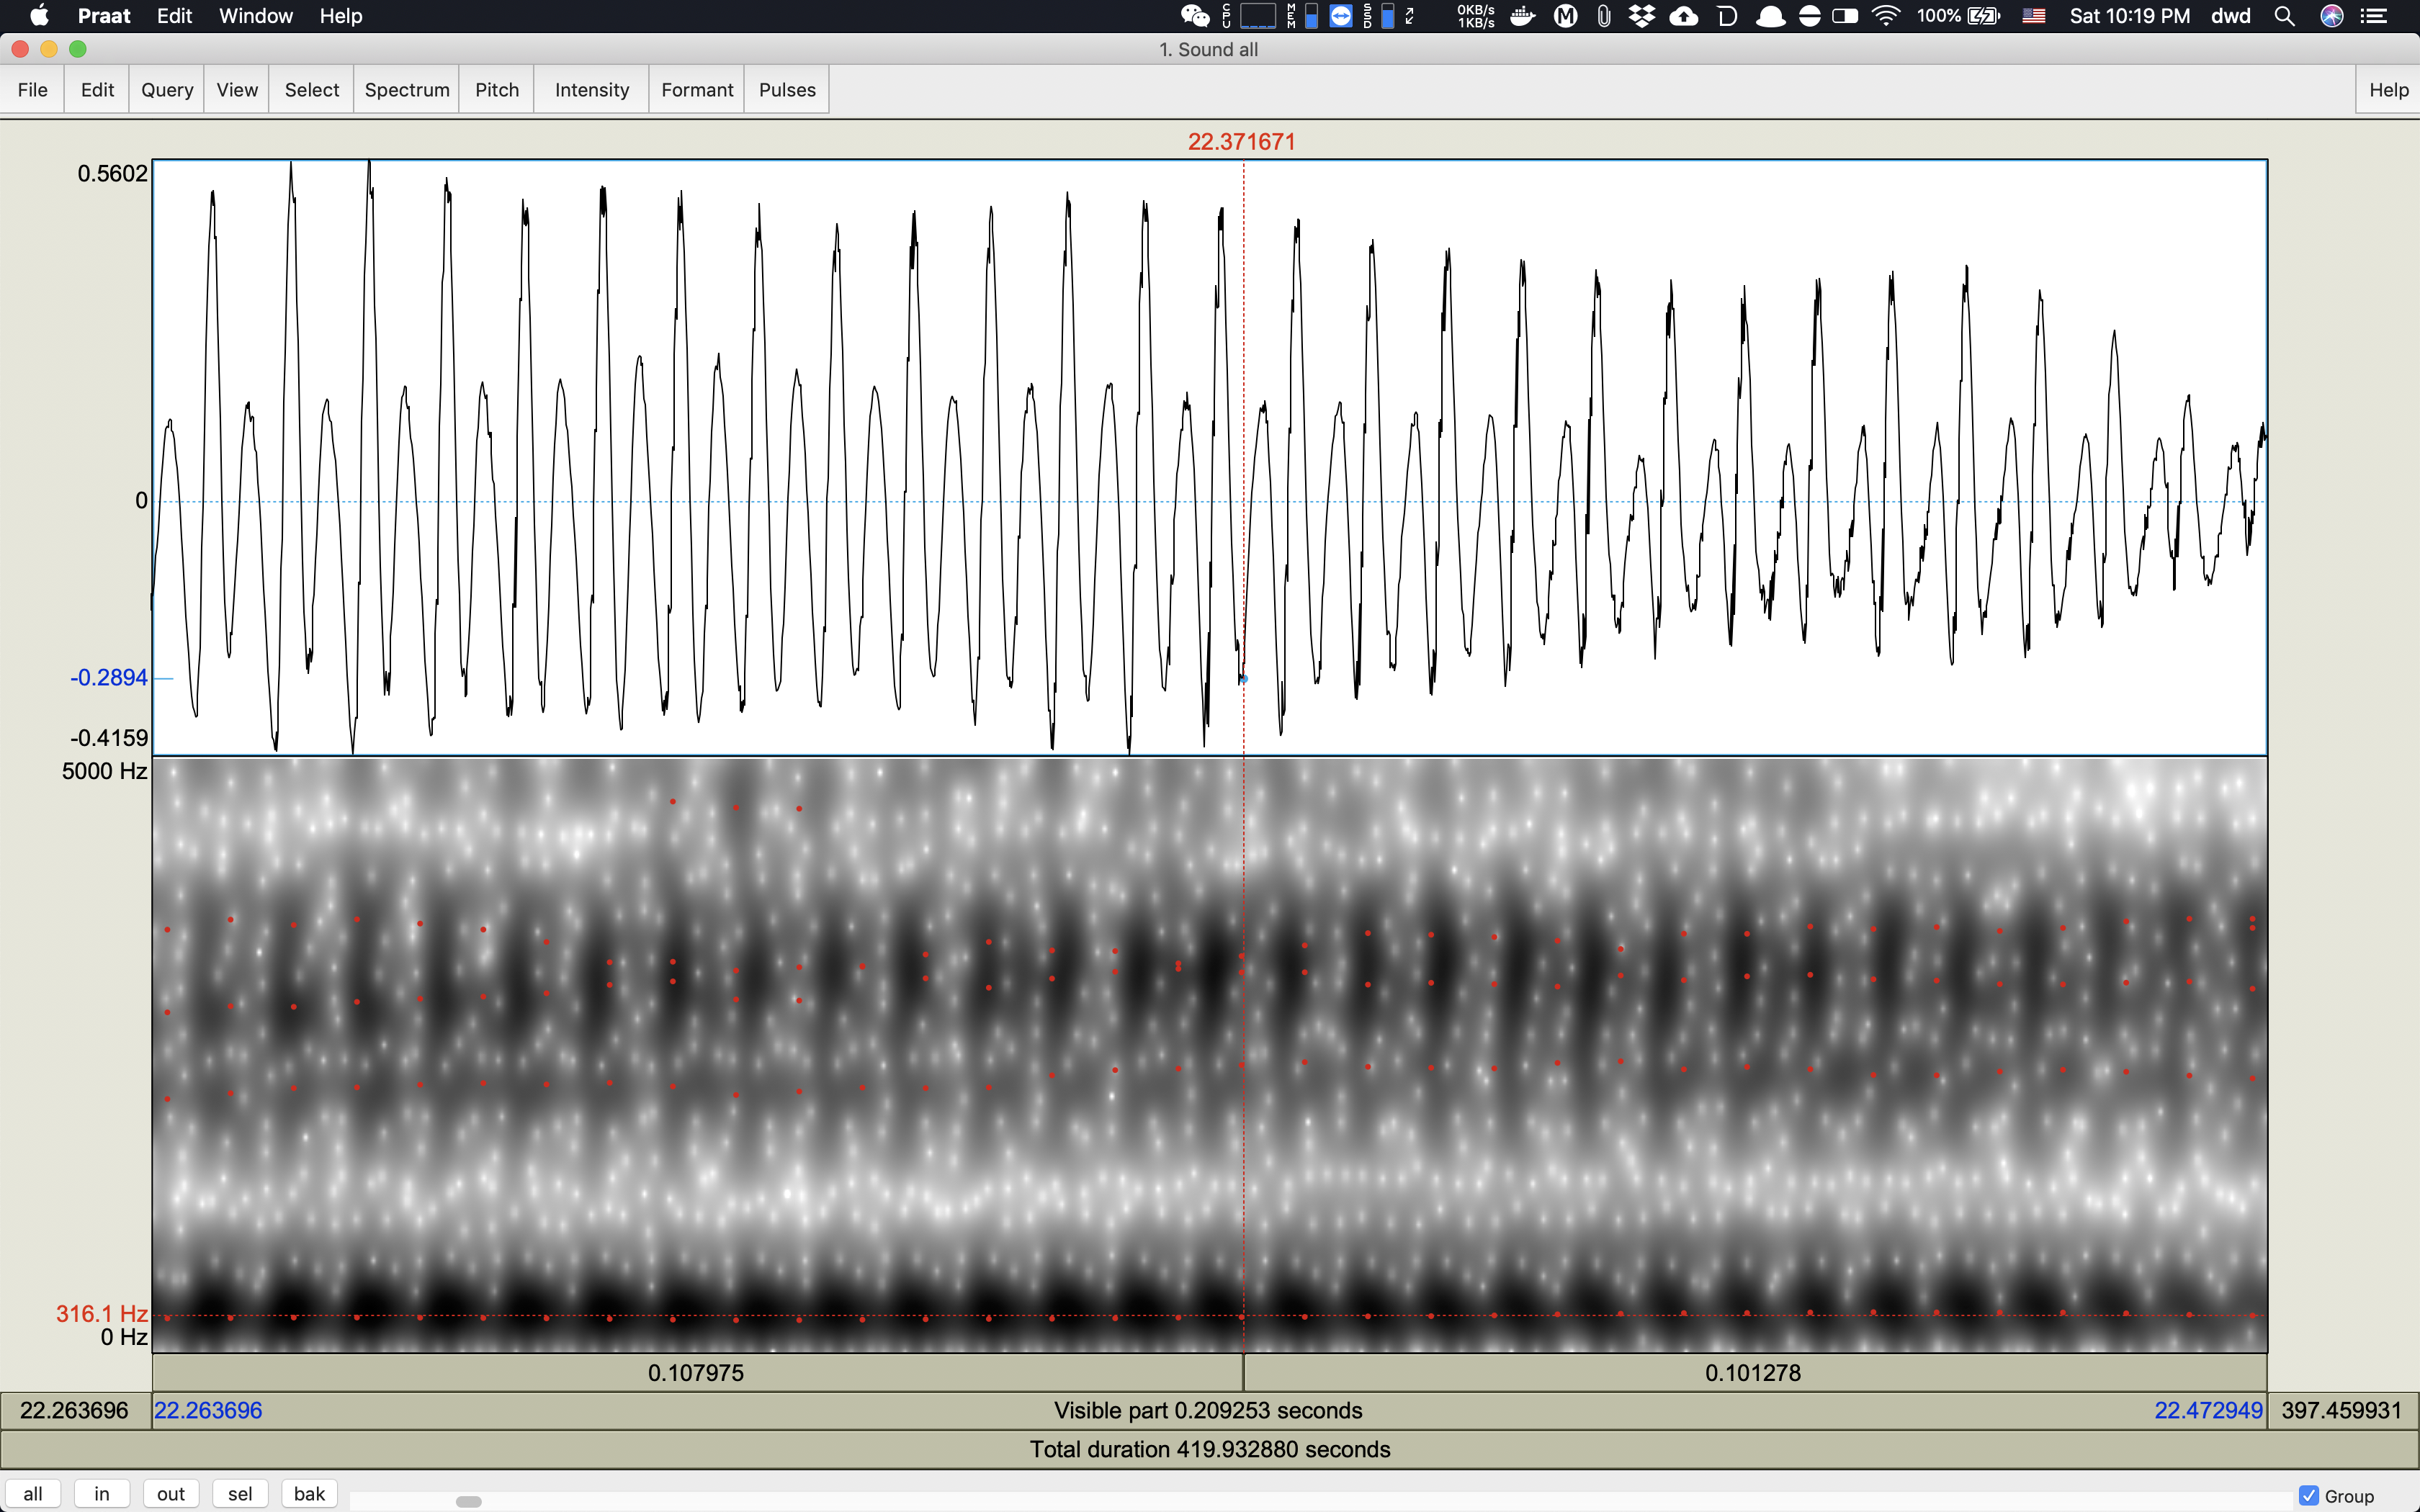
\includegraphics[scale=0.25]{imgs/vowel_i.png}
%     \caption{[i]}
% \end{figure}
% \begin{figure}[H]
%     \centering
%     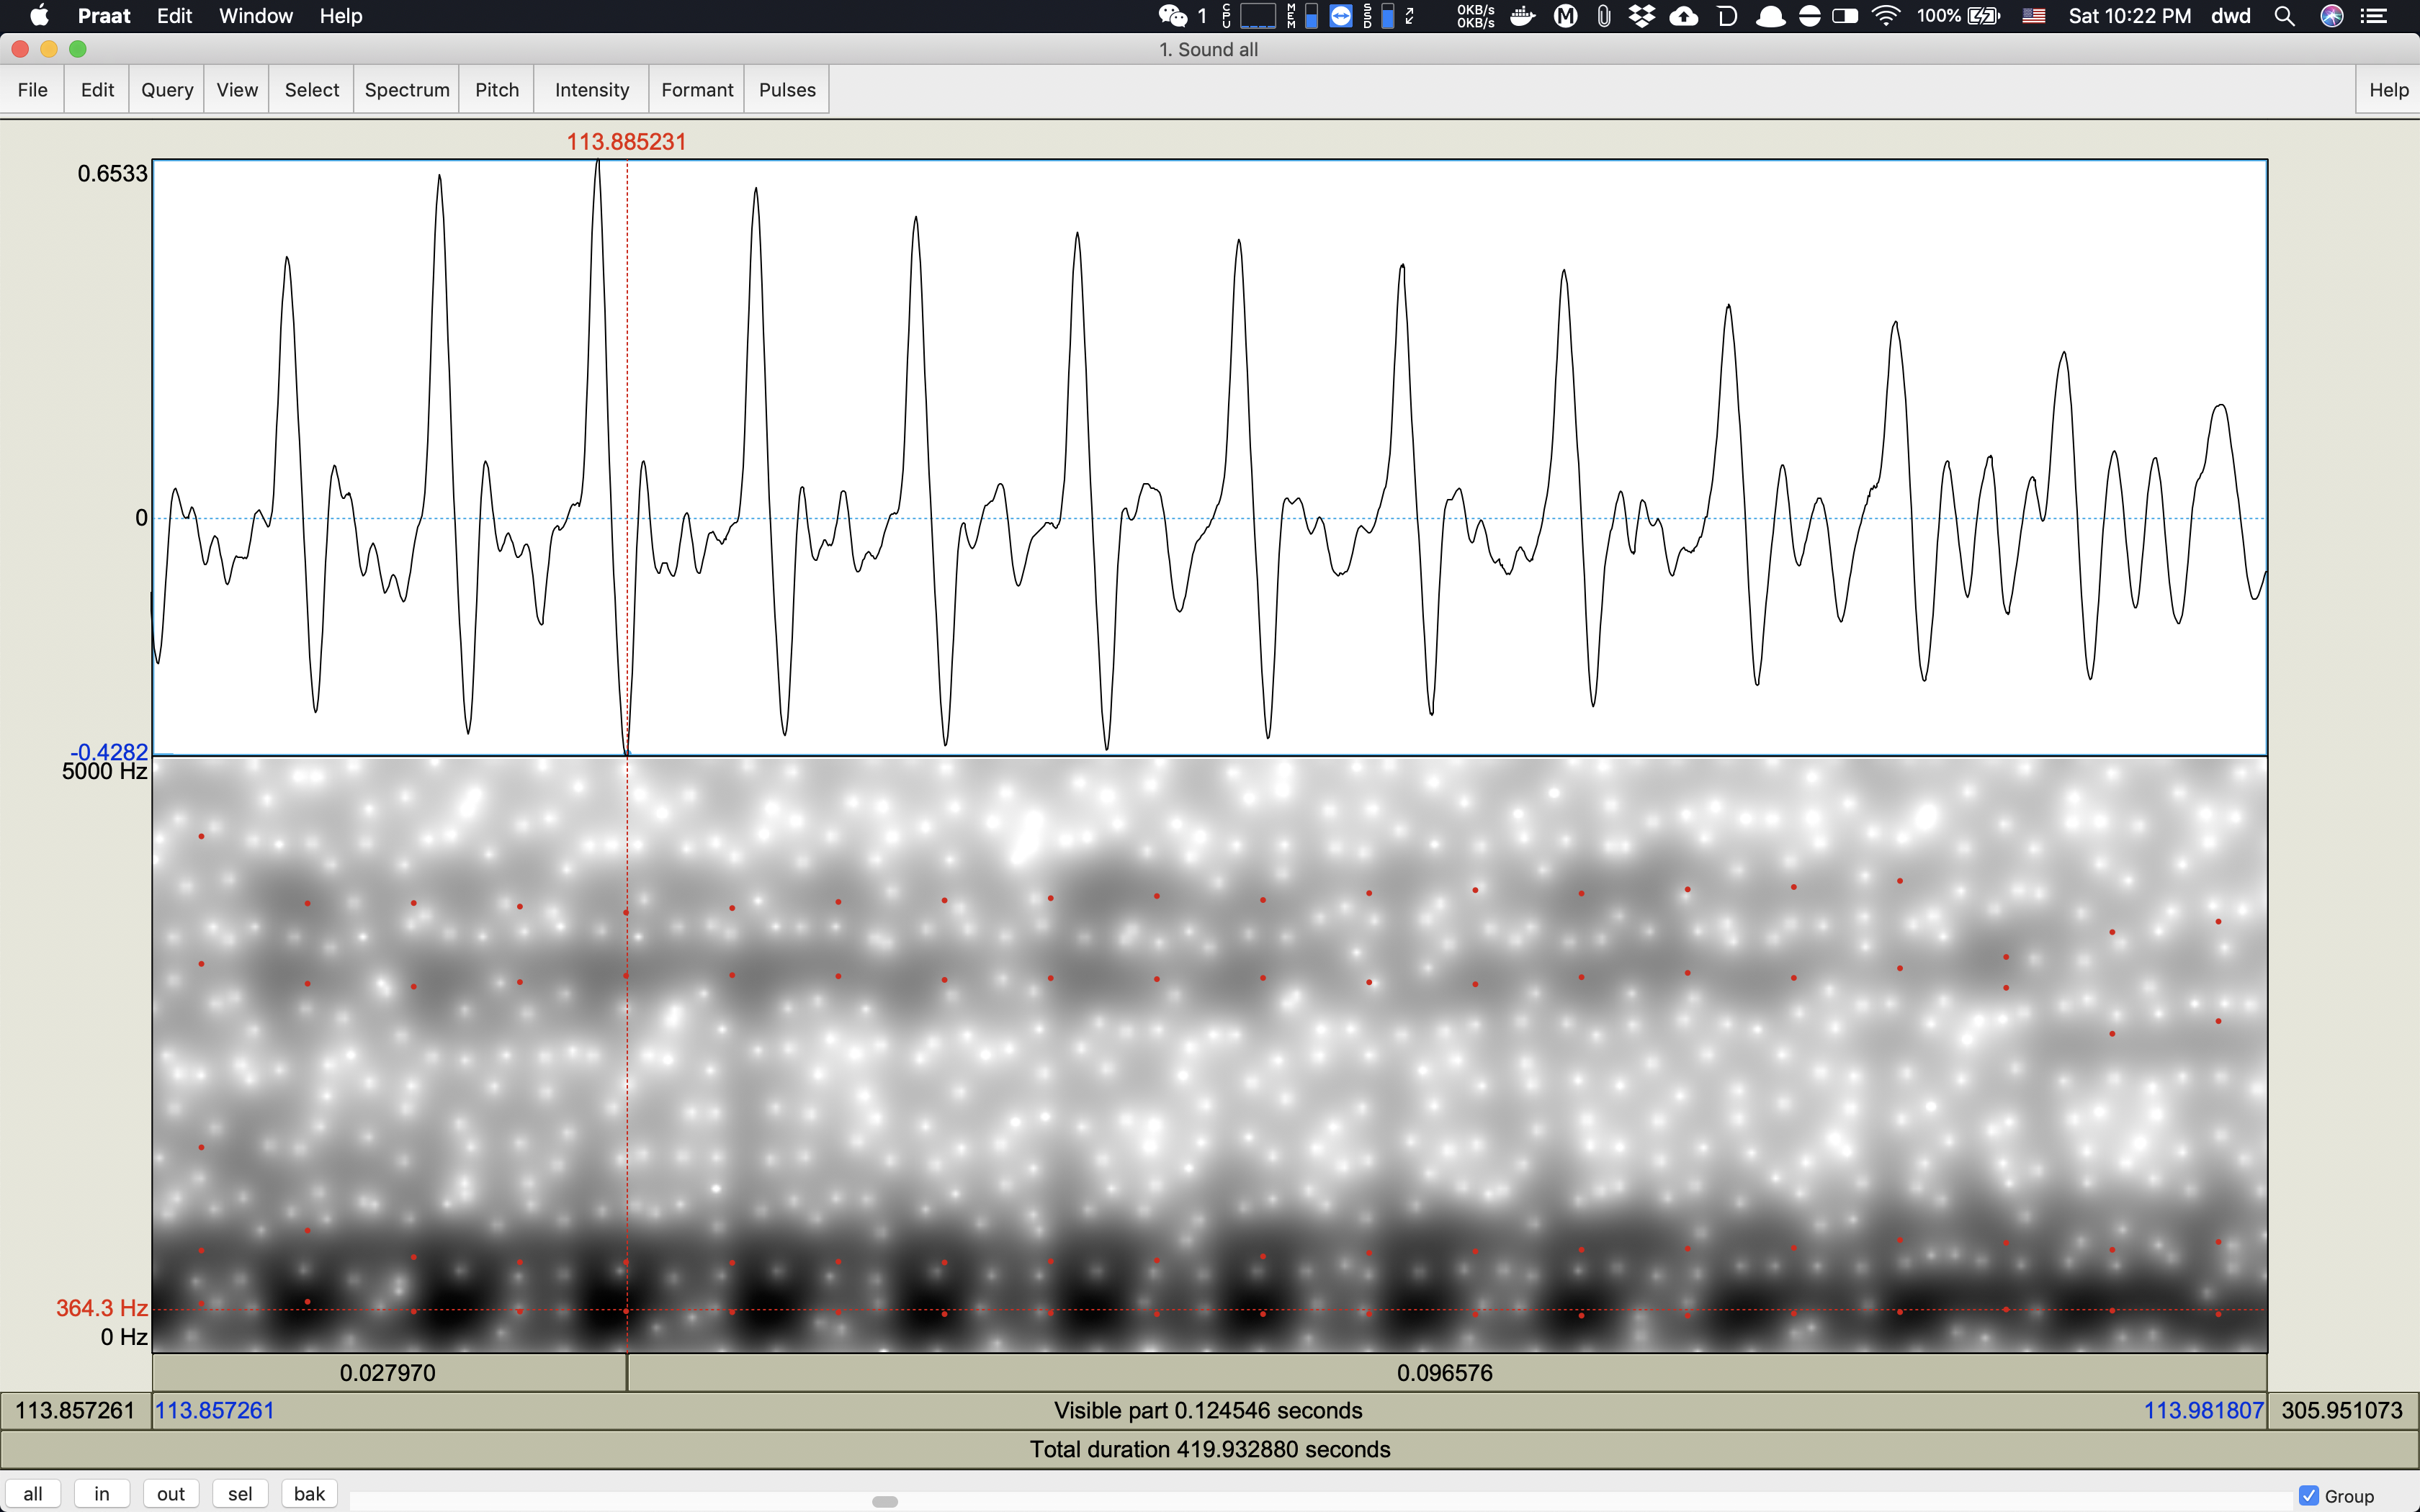
\includegraphics[scale=0.25]{imgs/vowel_u.png}
%     \caption{[u]}
% \end{figure}
% \begin{figure}[H]
%     \centering
%     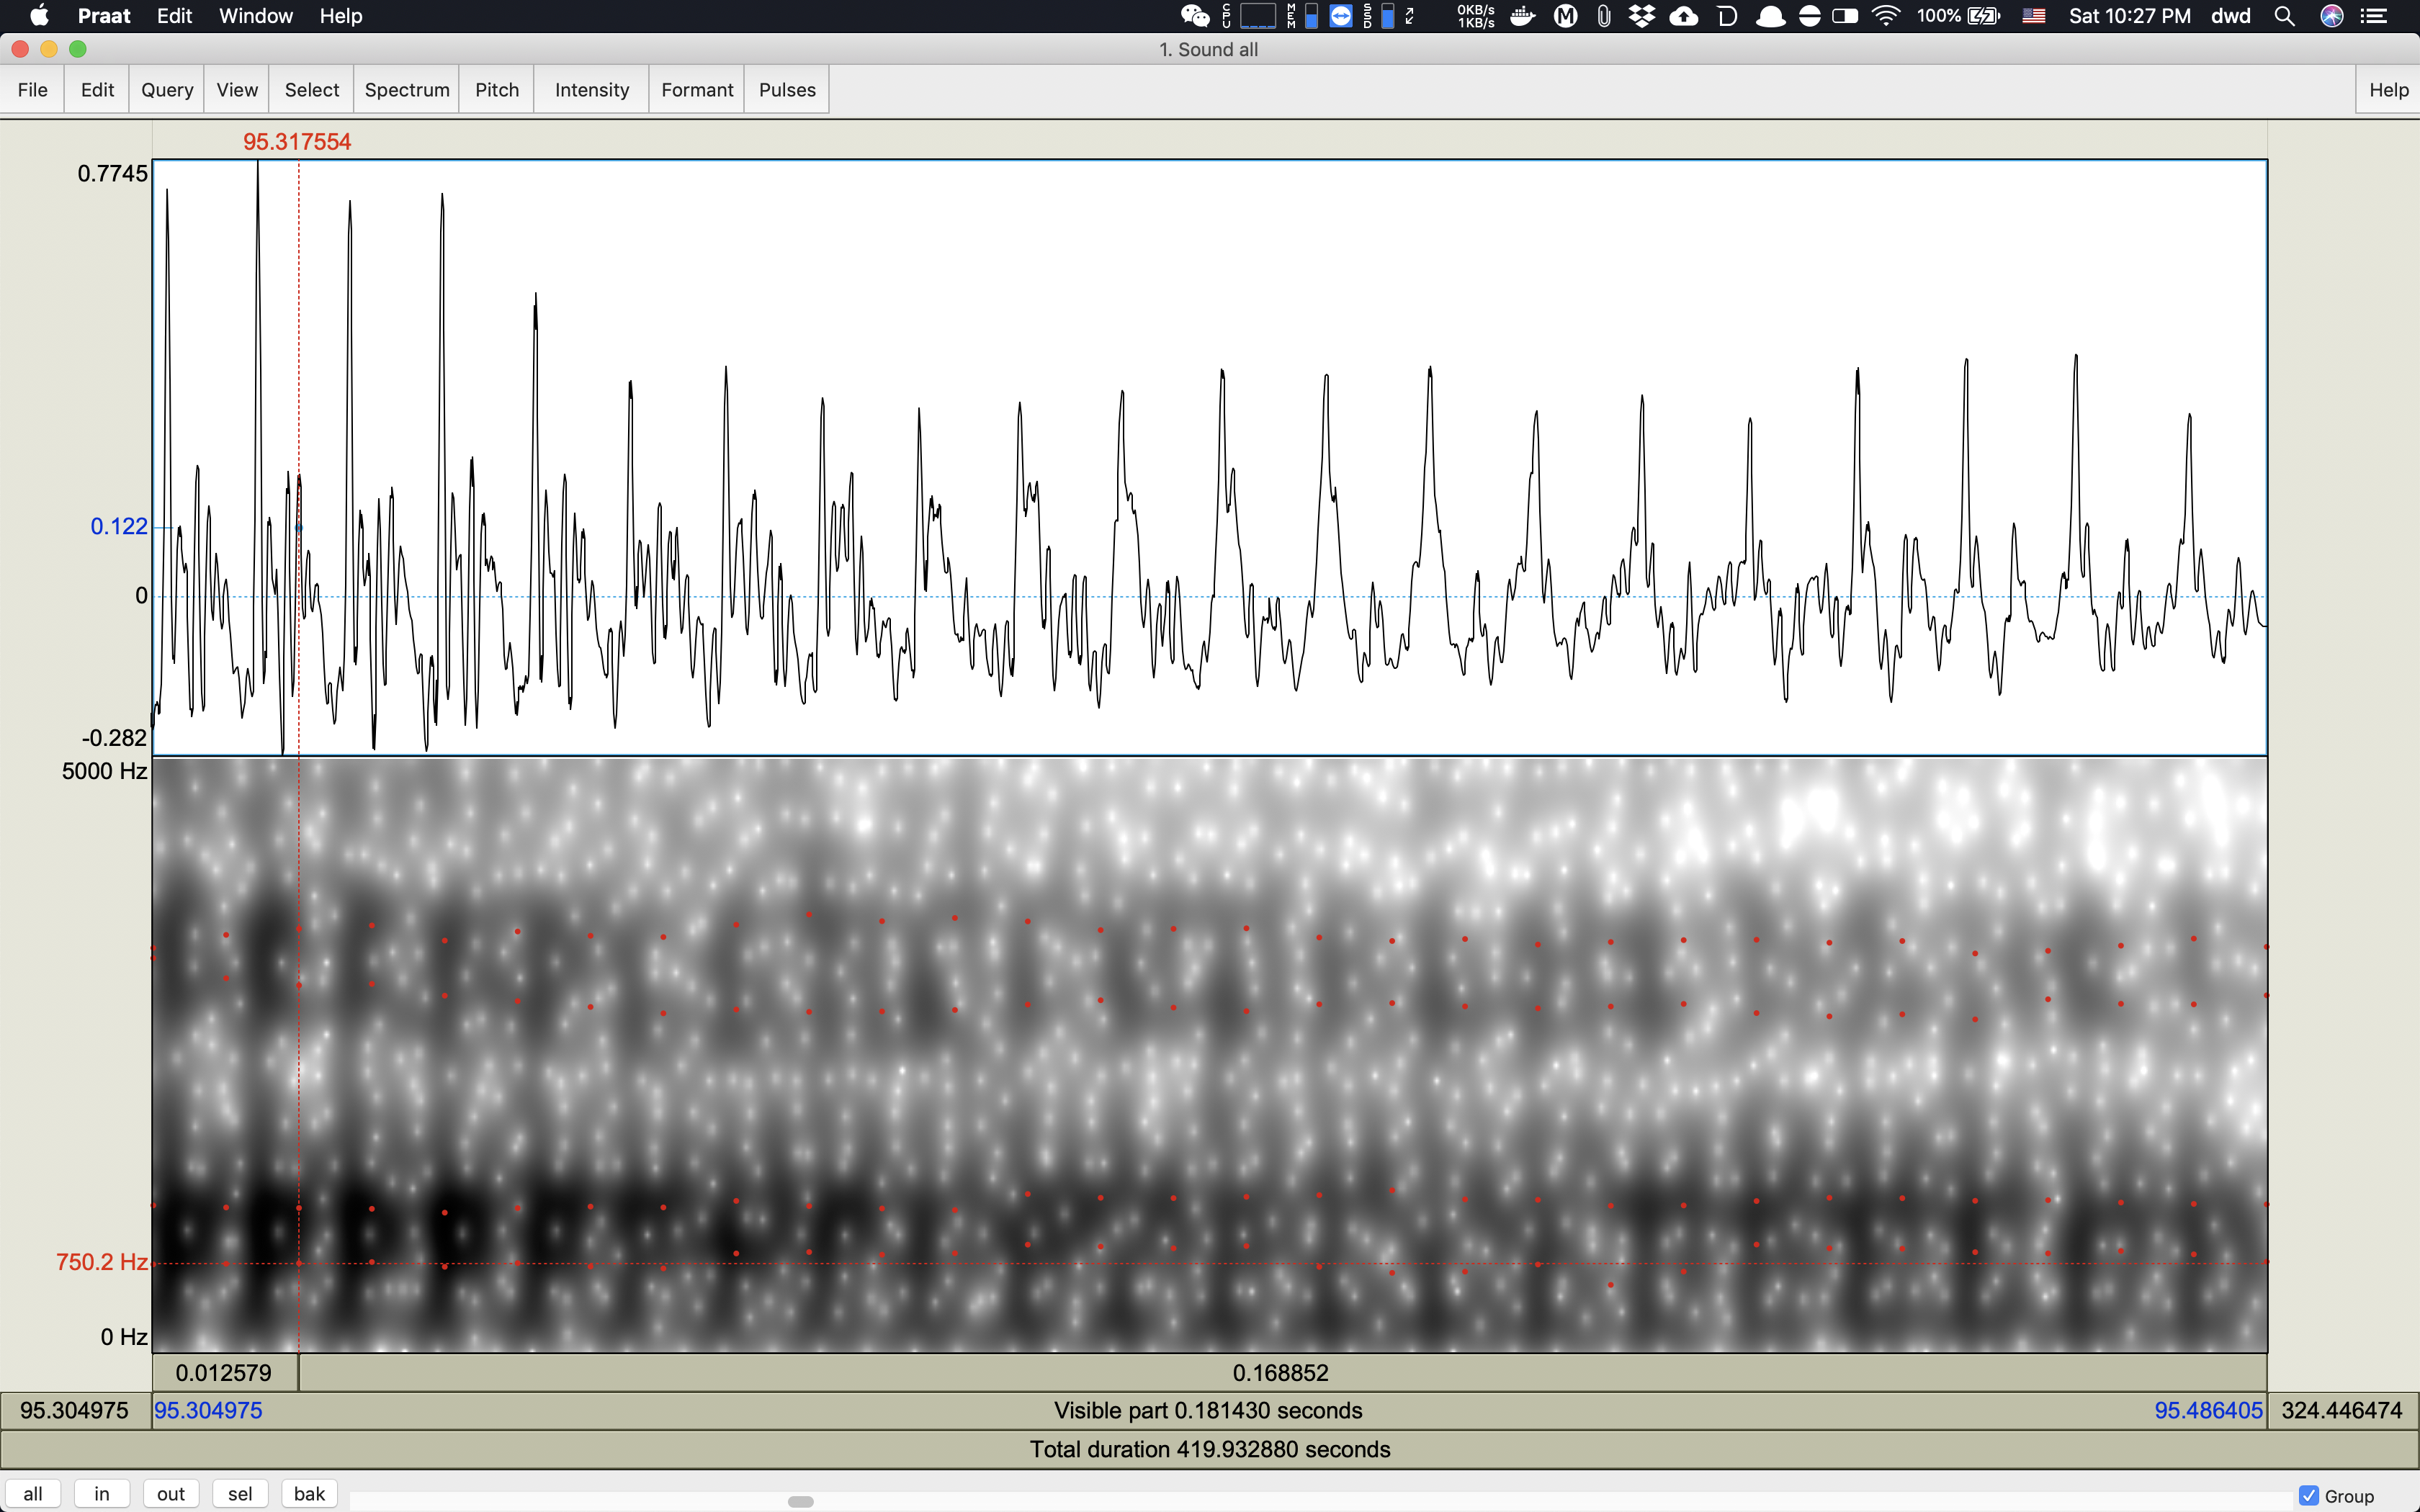
\includegraphics[scale=0.25]{imgs/vowel_a.png}
%     \caption{[a]}
% \end{figure}
% \begin{figure}[H]
%     \centering
%     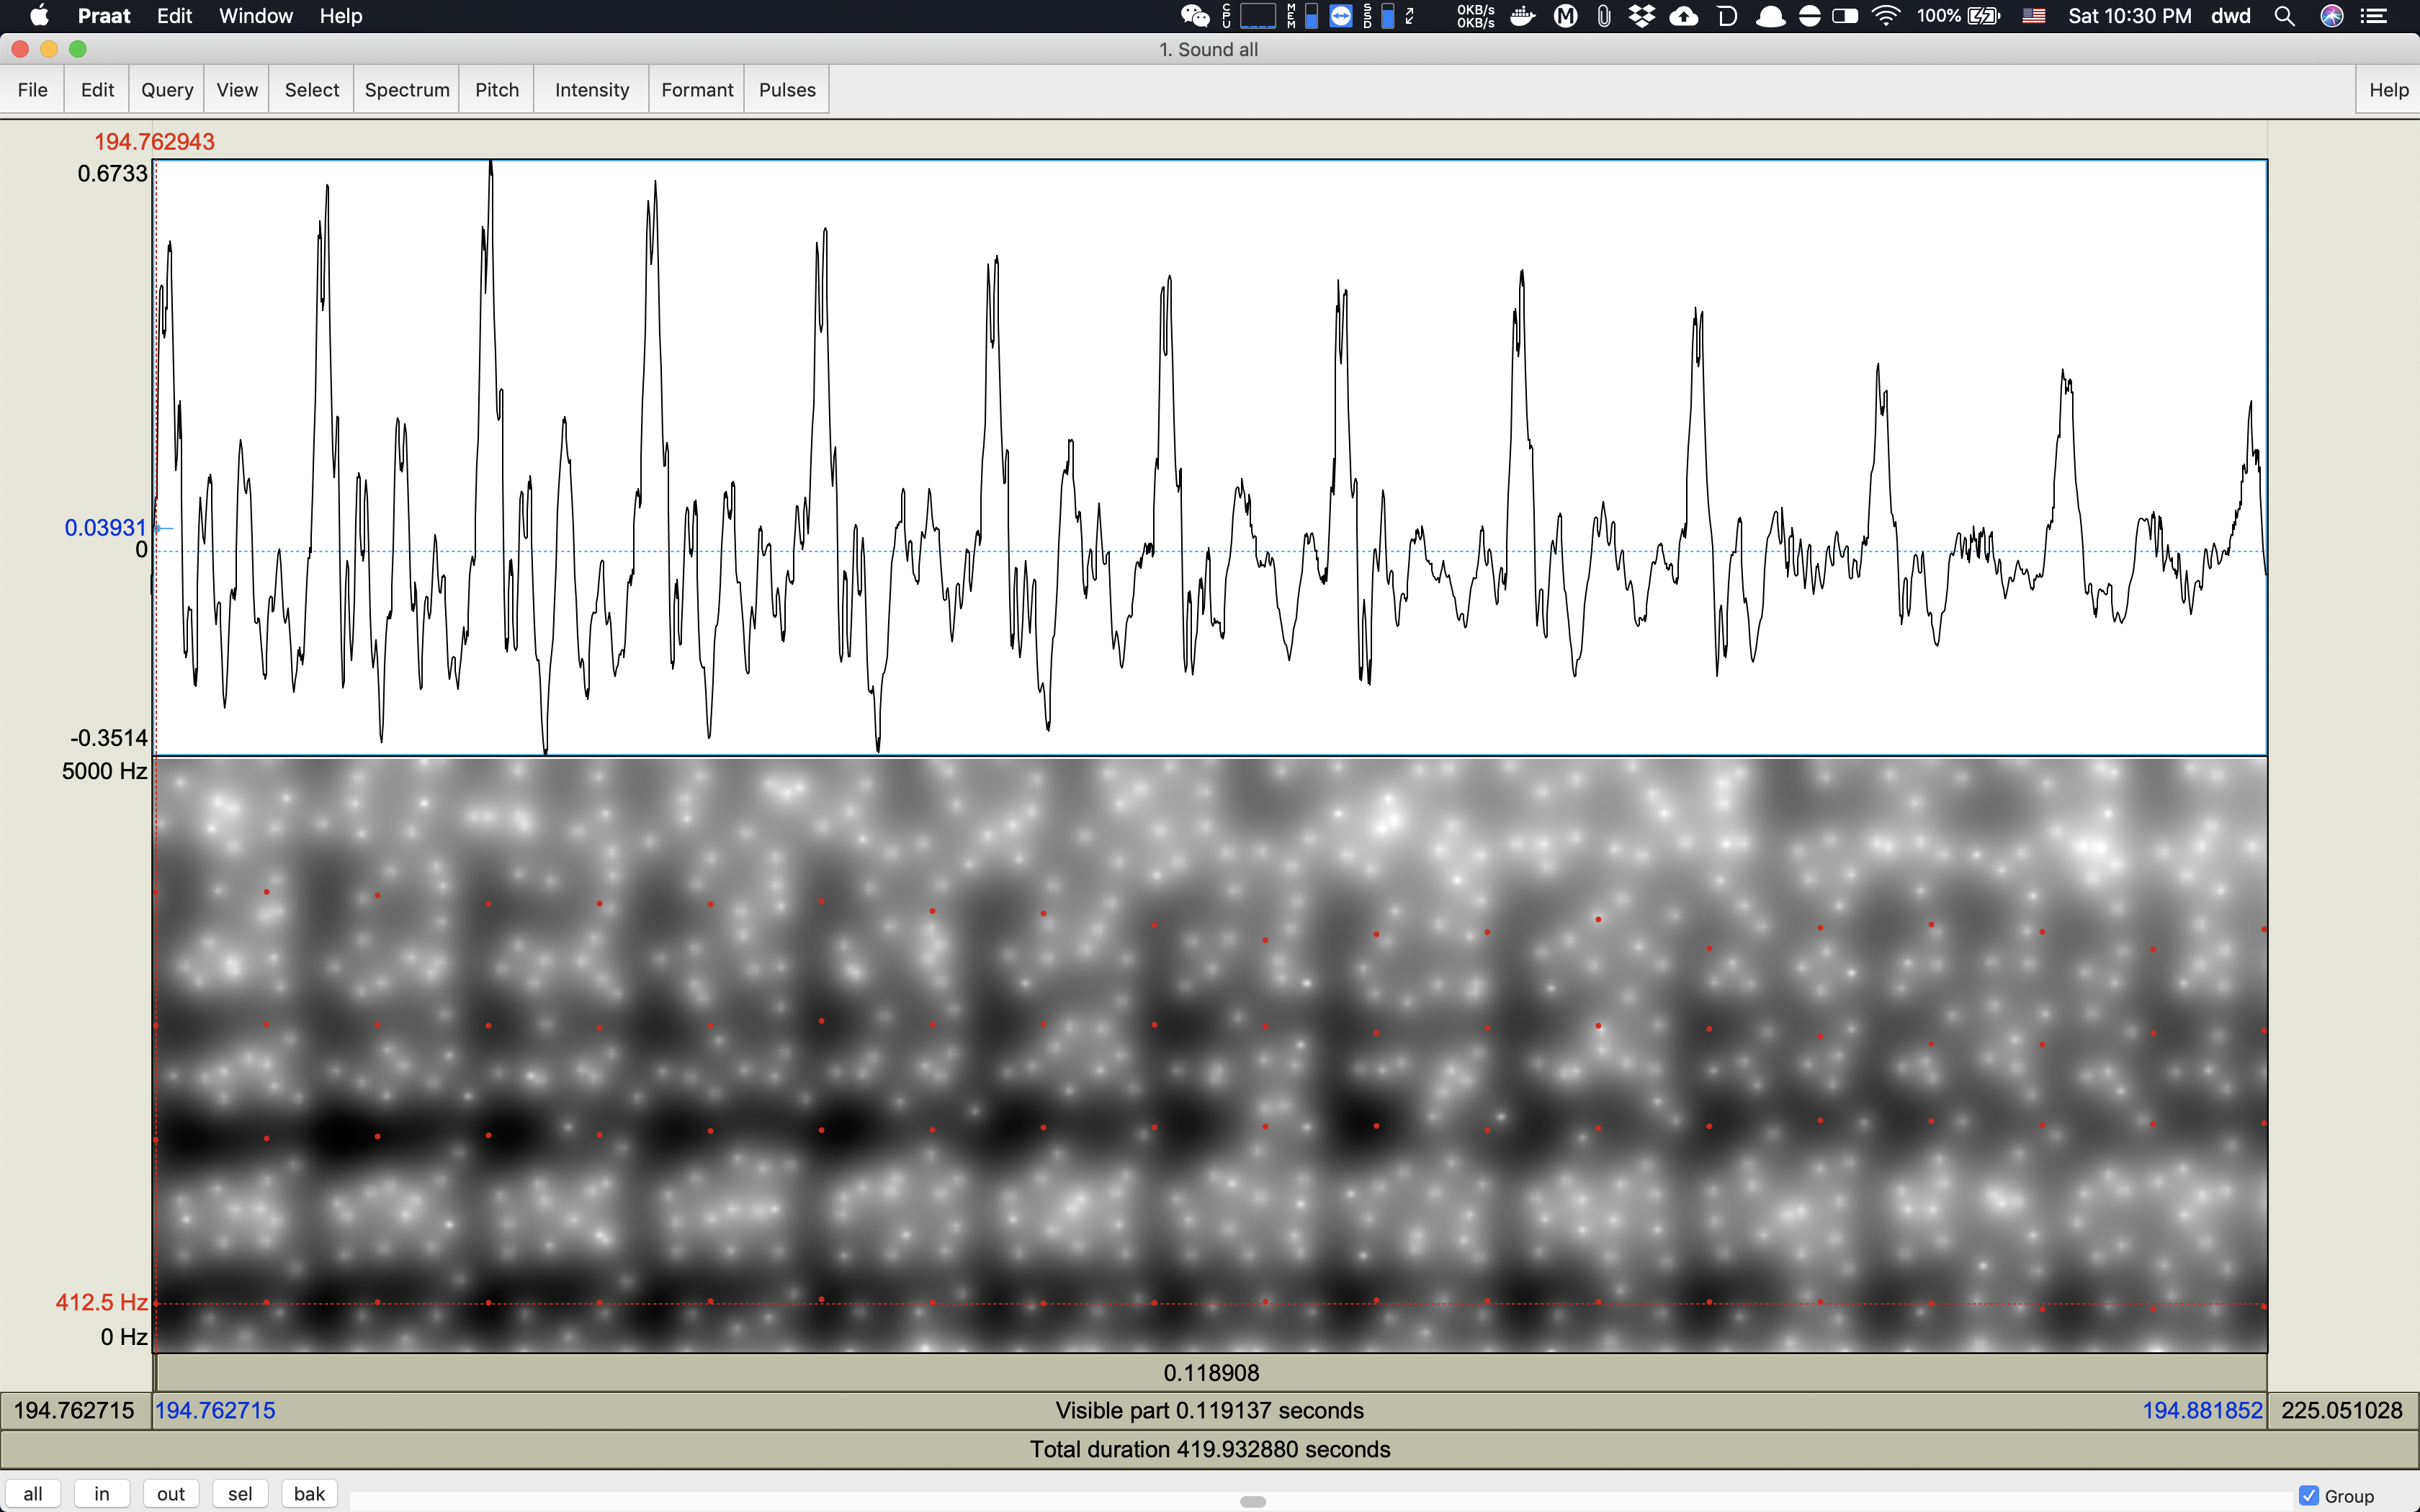
\includegraphics[scale=0.25]{imgs/vowel_e.png}
%     \caption{[e]}
% \end{figure}
% \begin{figure}[H]
%     \centering
%     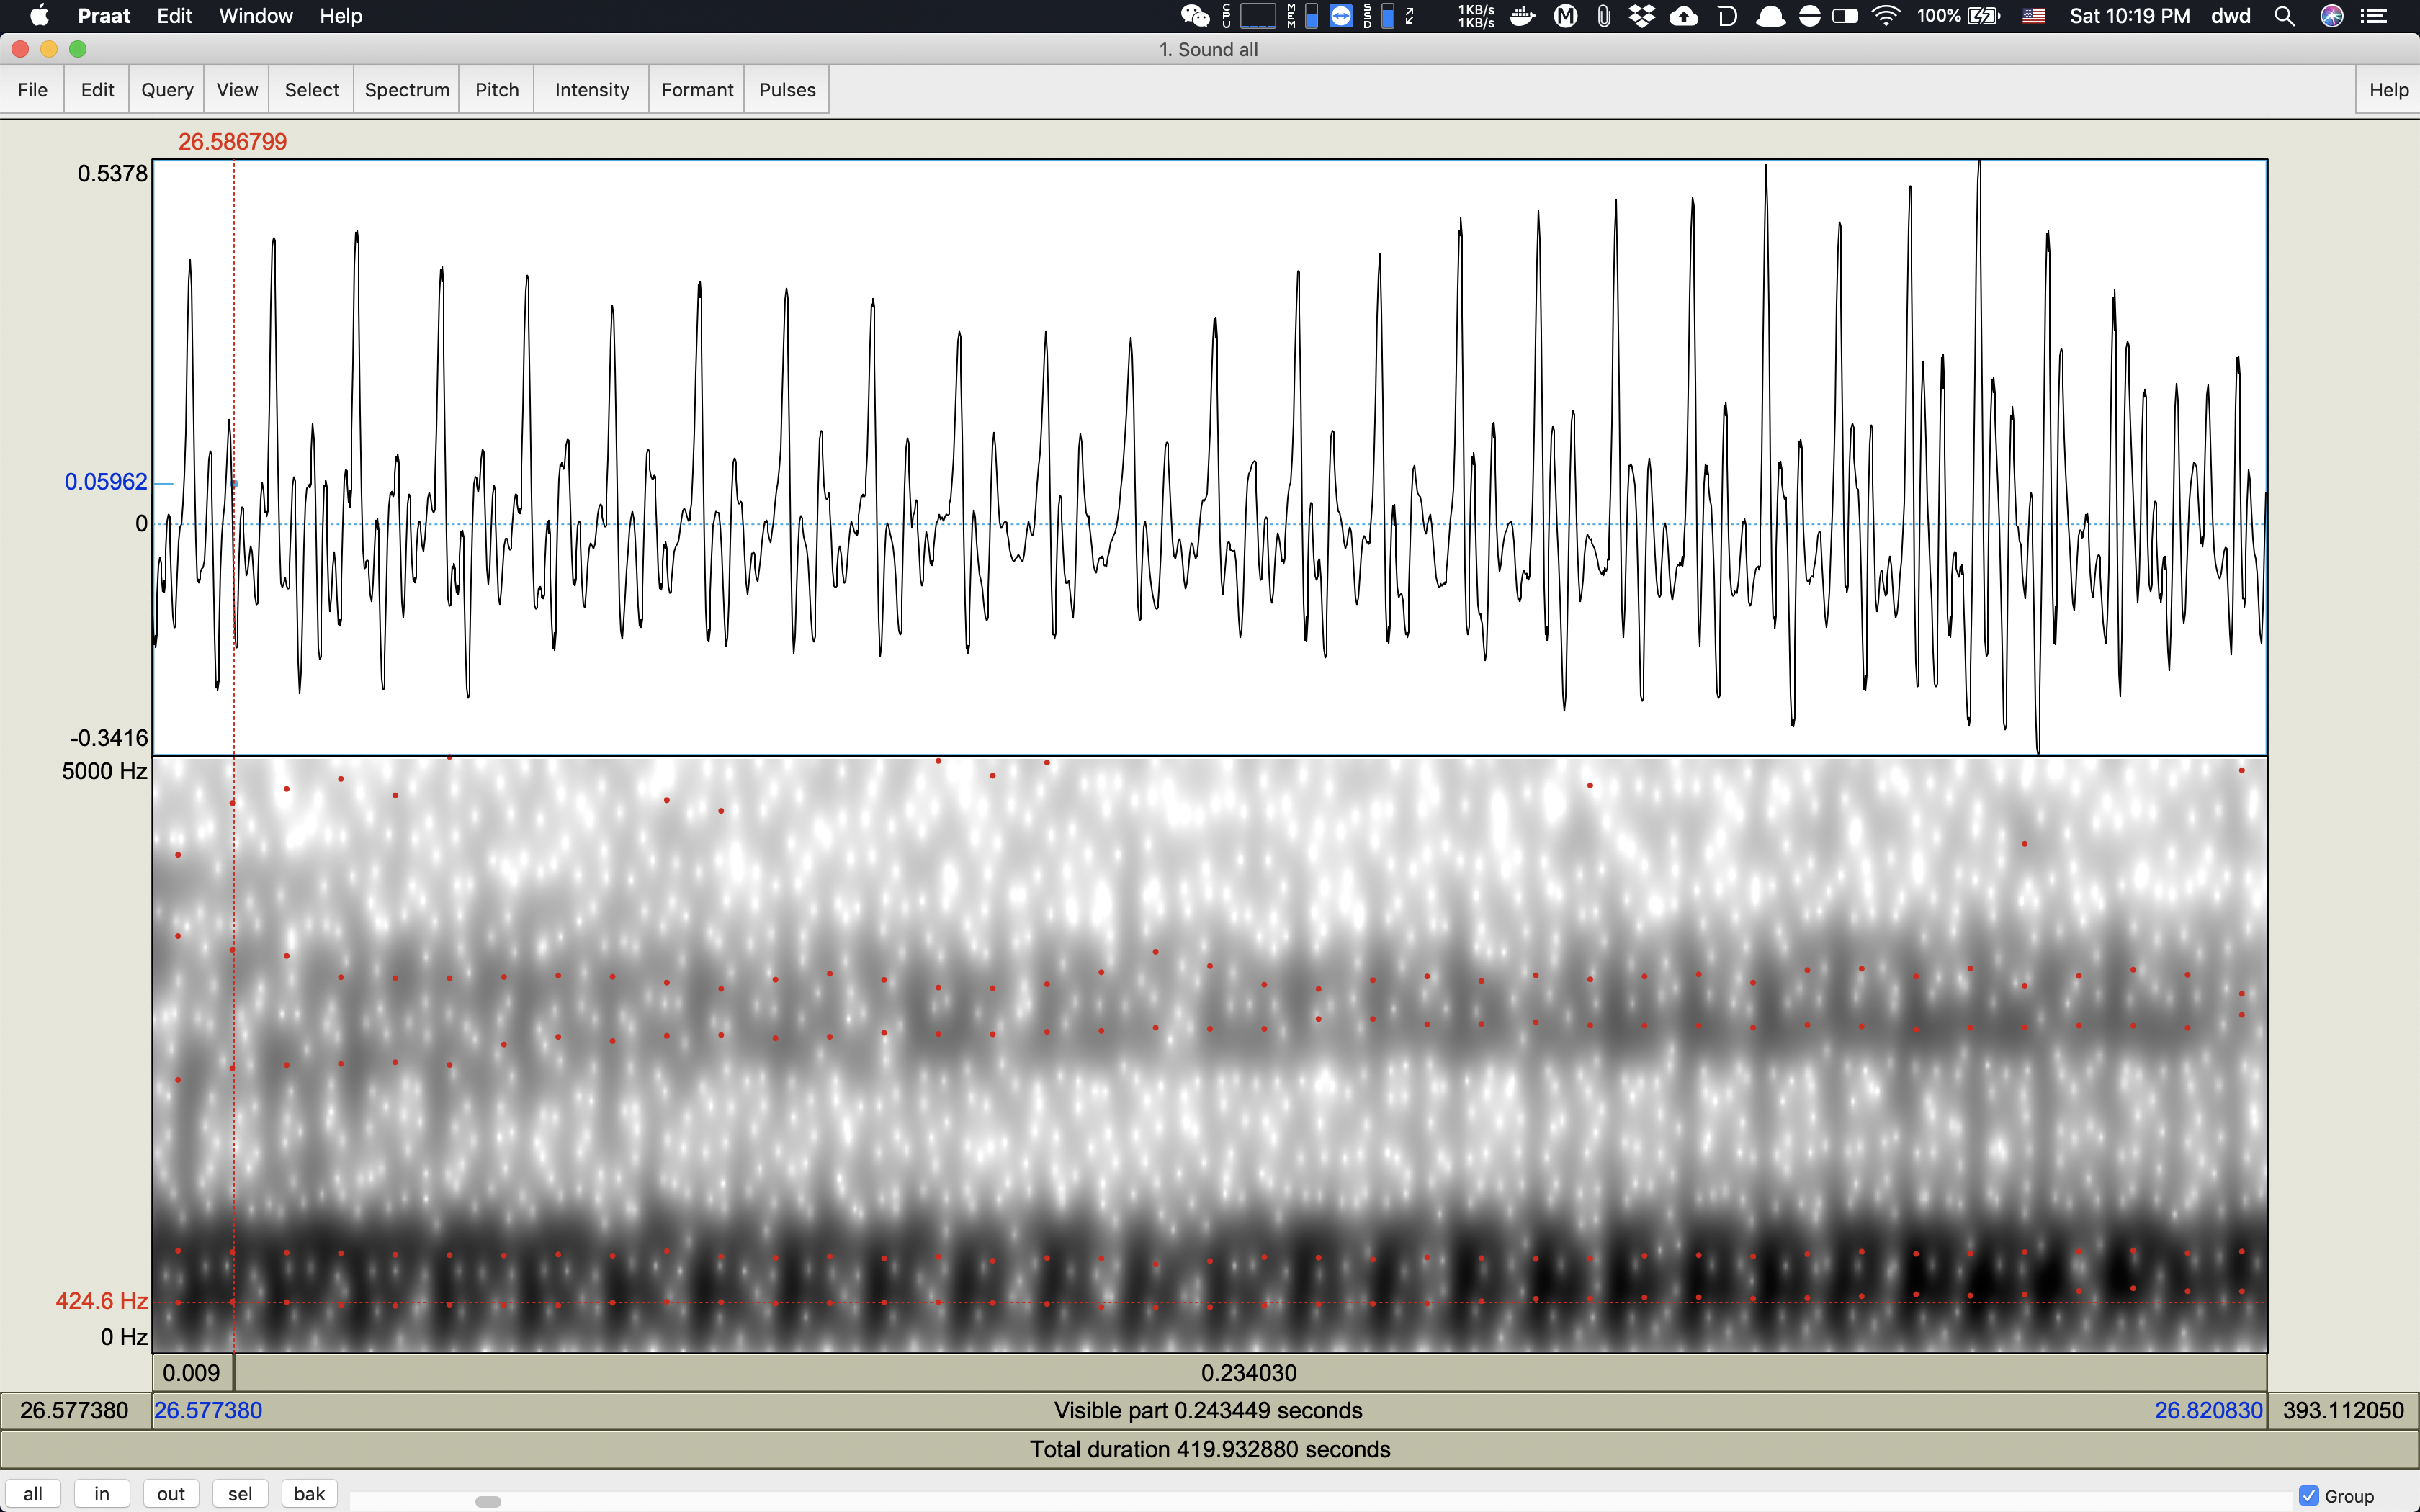
\includegraphics[scale=0.25]{imgs/vowel_o.png}
%     \caption{[o]}
% \end{figure}
% \begin{figure}[H]
%     \centering
%     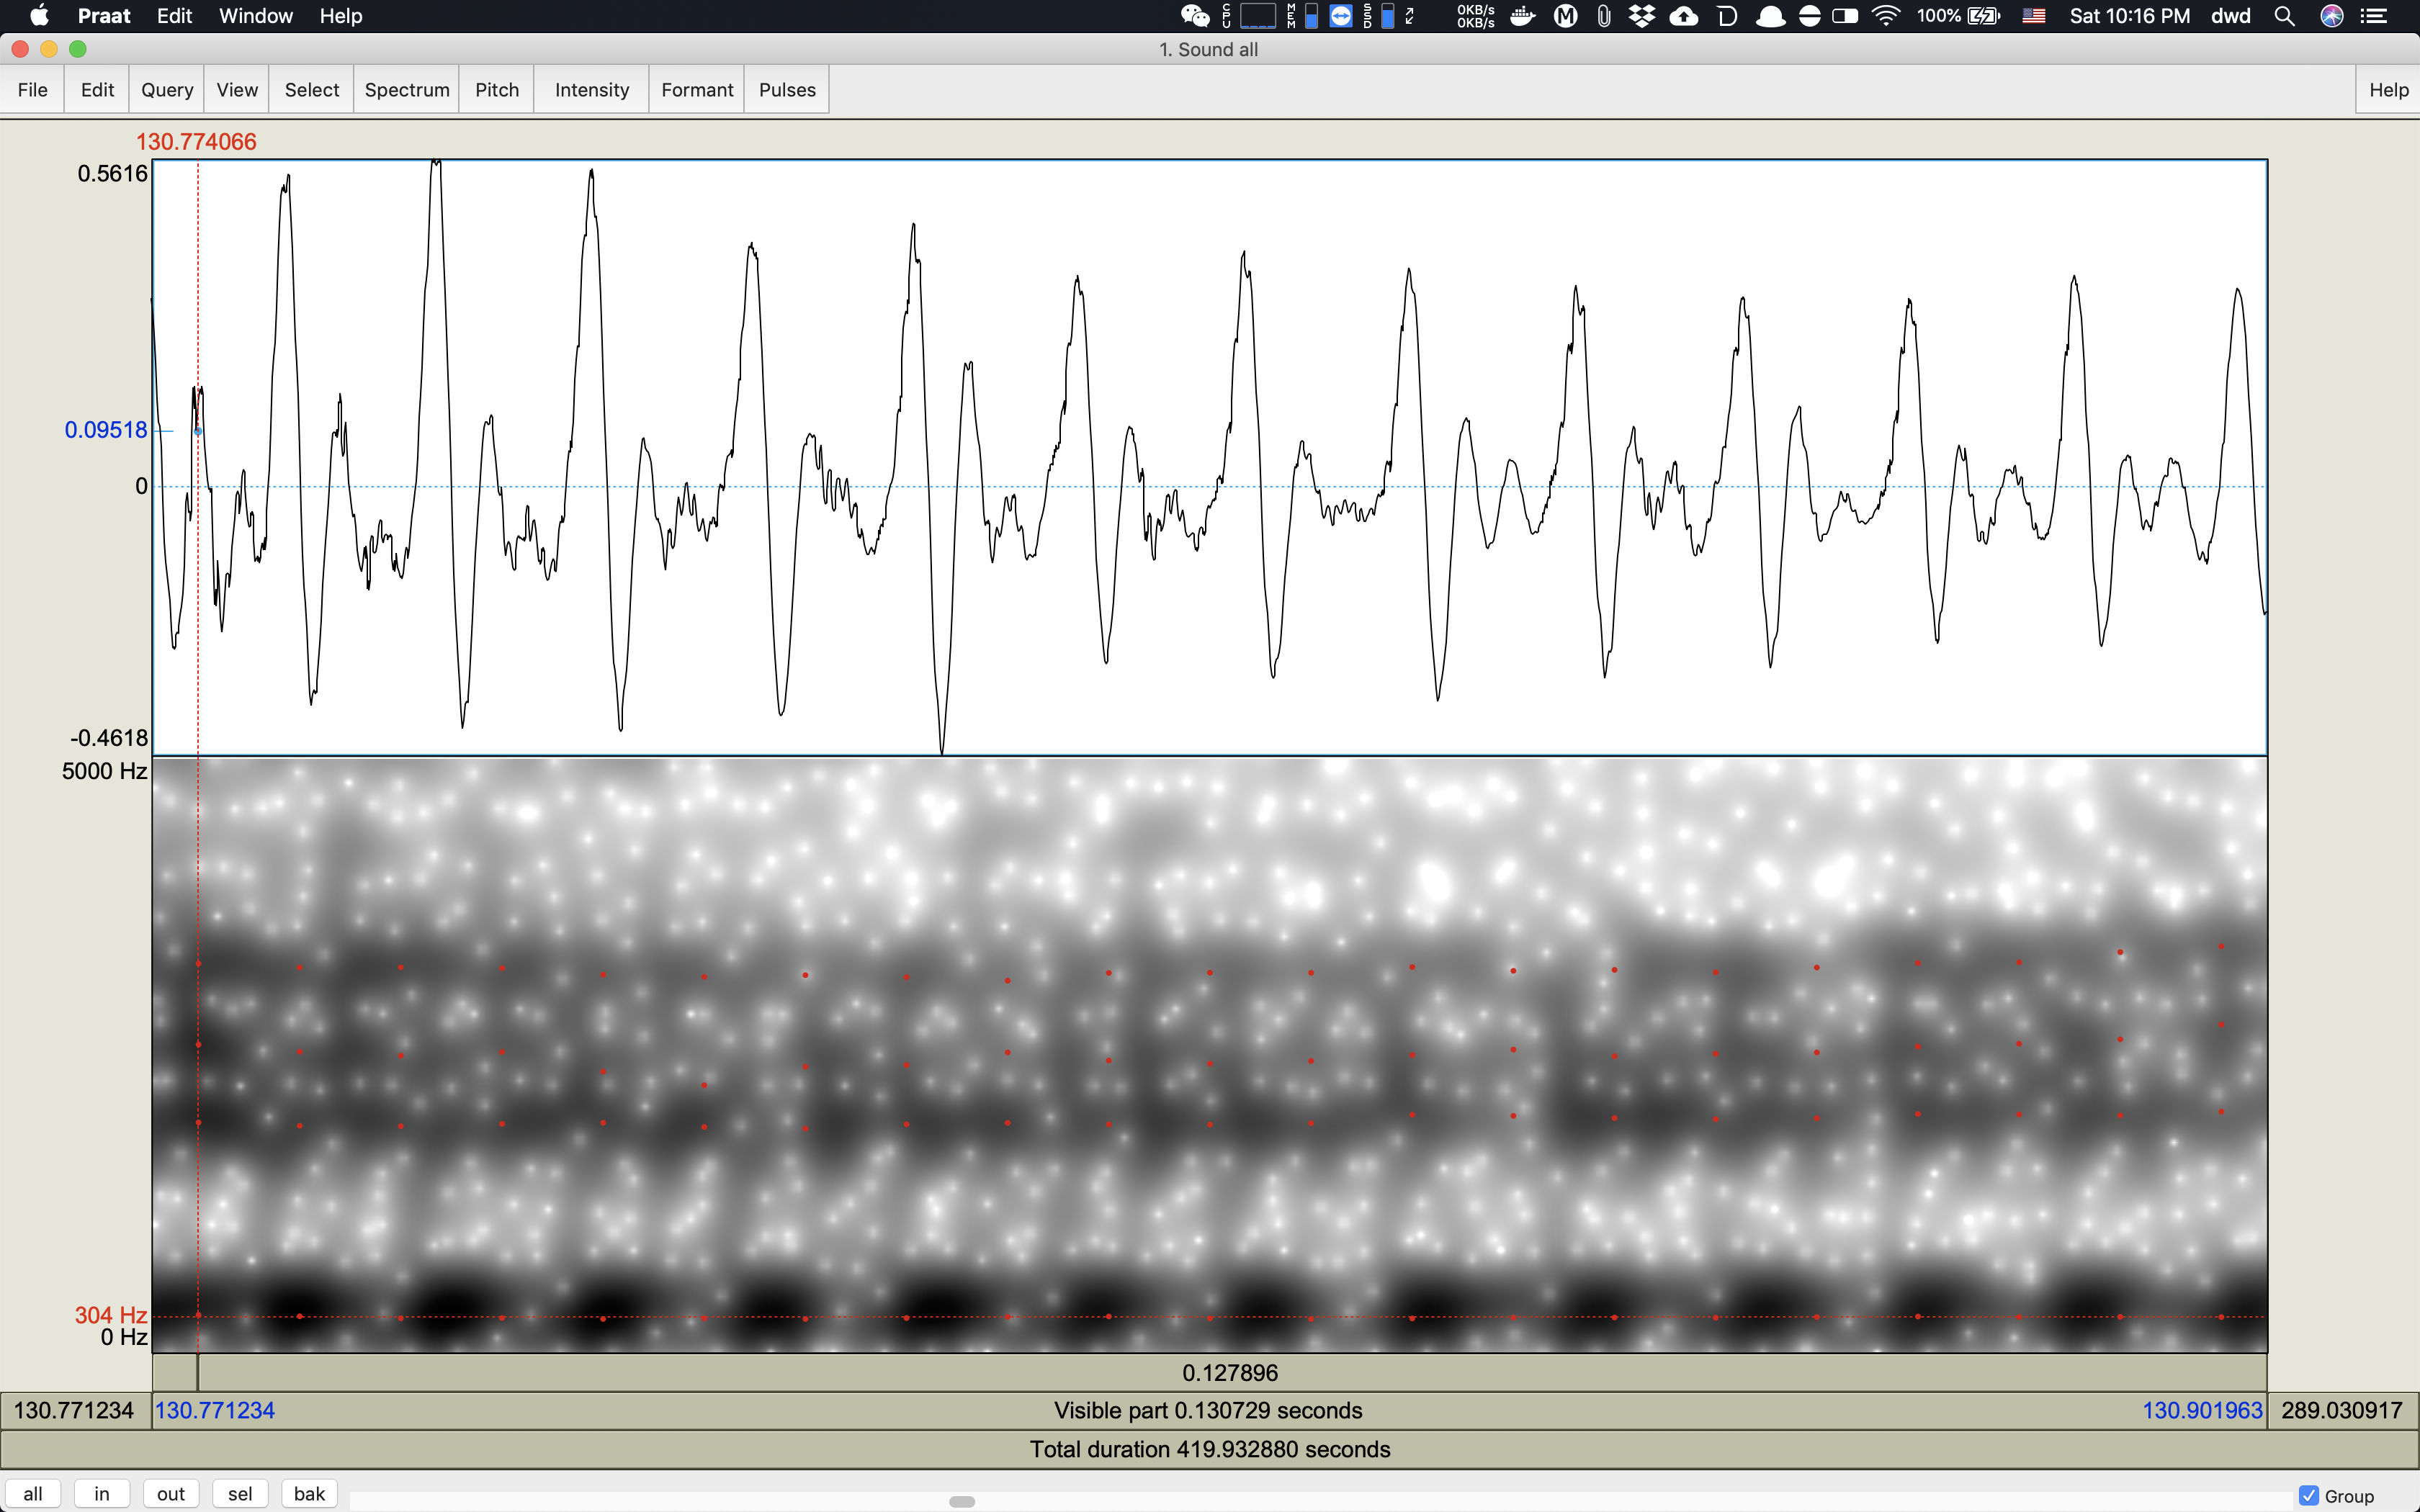
\includegraphics[scale=0.25]{imgs/vowel_y.png}
%     \caption{[y]}
% \end{figure}
% \begin{figure}[H]
%     \centering
%     \includegraphics[scale=0.25]{imgs/vowel_œ.png}
%     \caption{[œ]}
% \end{figure}

\subsection{Vowel Space Plotting}
\begin{figure}[H]
    \centering
    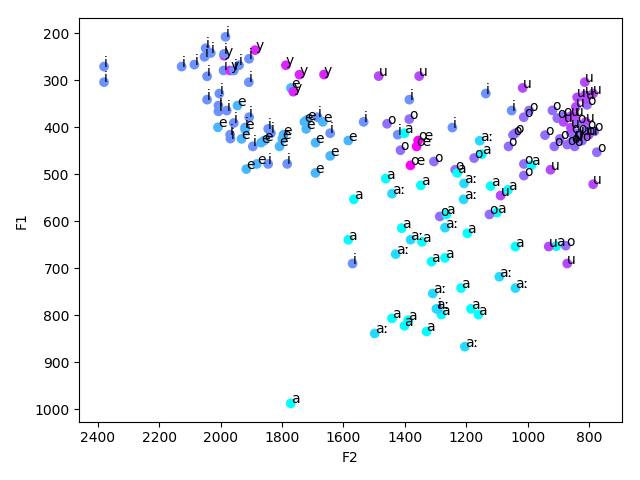
\includegraphics[scale=0.6]{imgs/vowelspace.png}
    \caption{vowel space of Cantonese (axes inverted)}
\end{figure}
The plotted vowel space bears some similarity with the vowel chart, at least the distribution of [i] (high and front), [a] (low and central), and [u] (high and back) is quite clear. Moreover, the location of [y] and [e] agrees well with their location in the vowel chart. Personally I think [u] and [o] are too close to each other, but it is still possible to see that [u] is higher than [o]. The position of [œ] is also quite ideal, though it appears to be more centralized than it should be. 

\subsection{Diphthong Movement}
\begin{figure}[H]
    \centering
    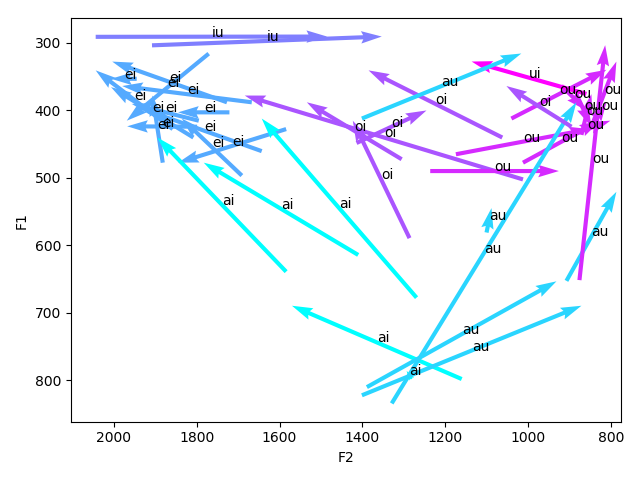
\includegraphics[scale=0.6]{imgs/diphthong_movement.png}
    \caption{diphthong movement of Cantonese (axes inverted)}
\end{figure}
The start of an arrow corresponds to the F1 and F2 value of the first phoneme in a diphthong, while the end of an arrow corresponds to that of the second phoneme. As we can see, the direction of arrows of a diphthong has a certain level of consistency.

\subsection{Vowel Variety and Symmetry}
According to the standard of WALS, Cantonese has a large vowel quality inventory (7 > 6). All vowels are peripheral. The vowel quality inventory is asymmetrical and the peripheral structure should be characterized as ``left'' since there are more front vowels than back vowels. 

\end{document}